\chapter{Referencial Te�rico}
\label{cha:refTeorico}
Apresentar todas as tecnolonologias utilizadas para o desenvolvimento do trabalho

\section{Entrada de S�mbolos e Siglas}
Para fazer a entrada de um s�mbolo, $\backslash$s�mbolo\{\simbolo{$\sigma$}{Descri��o}\} \{sigma\} � a forma correta. E, para definir uma sigla, $\backslash$sigla\{\sigla{ABNT}{Associa��o Brasileira de Normas T�cnicas}\} \{Descri��o\} deve ser utilizado.

Obs.: Quando a sigla ou o s�mbolo aparecerem novamente no texto, n�o repita o comando, para que a sigla ou s�mbolo n�o se repita na lista correspondente.

\section{Introdu��o � tecnologia X}


Inserindo uma referencia da tecnologia x \cite{ref}.


Exemplo para inserir figura. Figura \ref{fig:nomeParaRef}.


\begin{figure}[!htb]
	\centering
	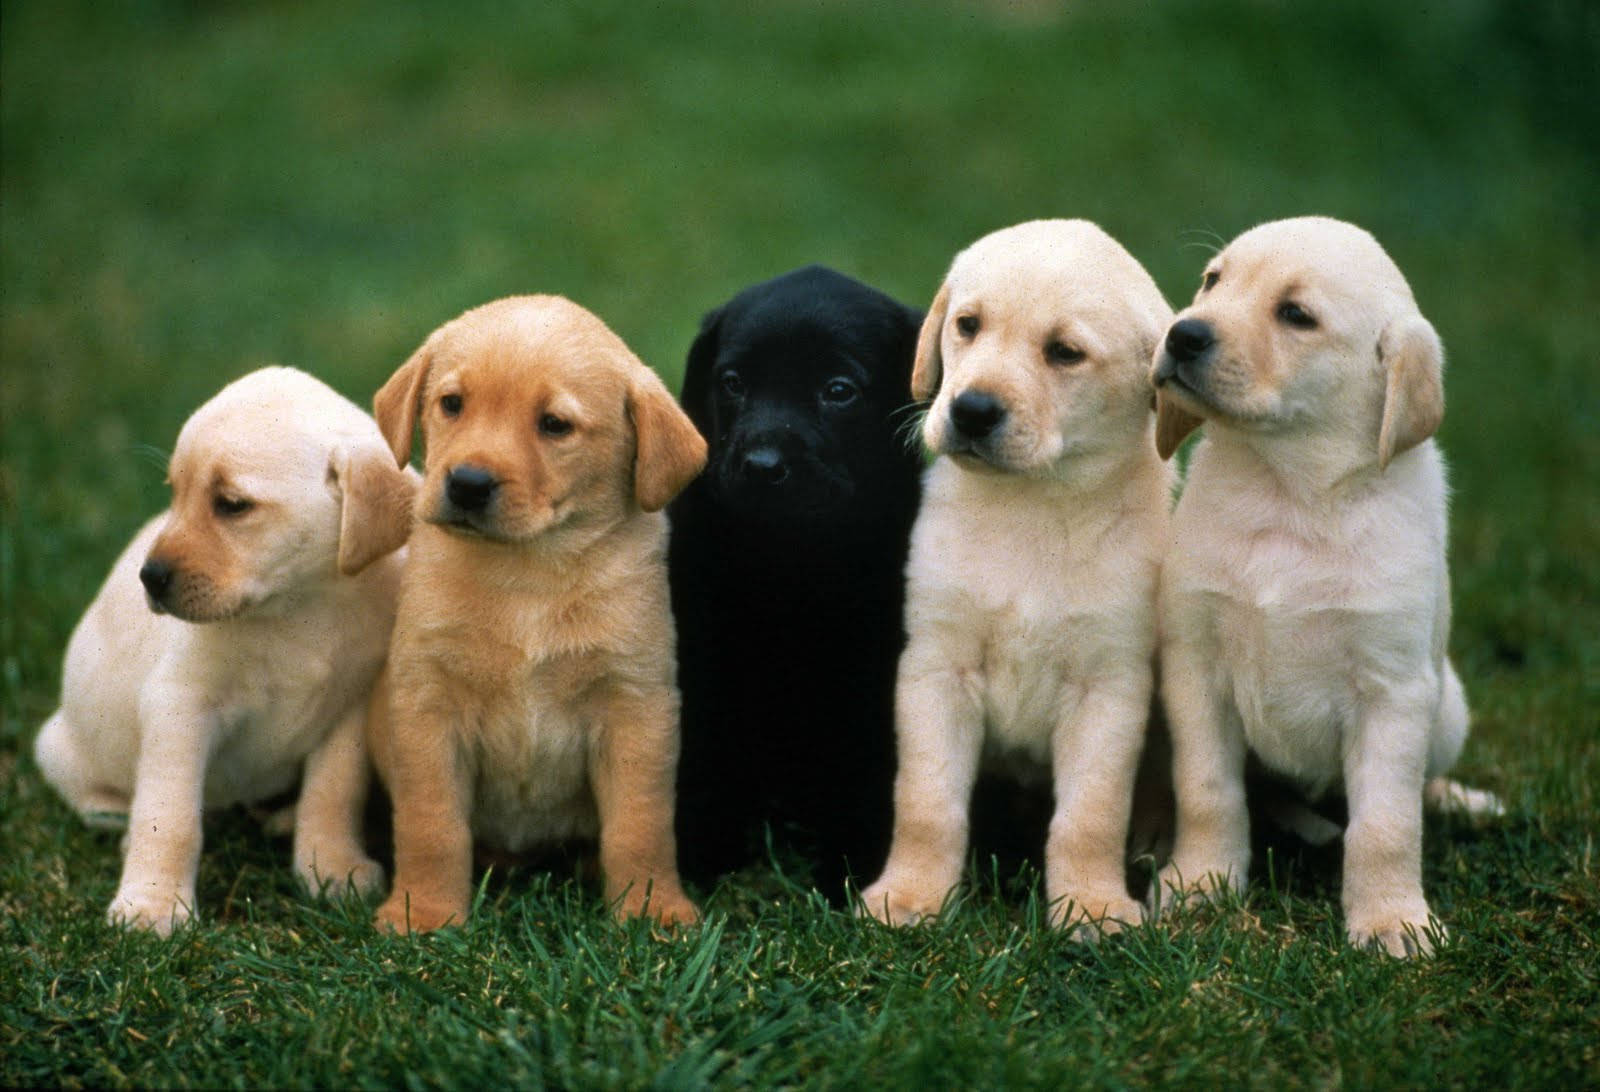
\includegraphics[width=0.45\textwidth]{../5_figuras/fig1}
	\caption{T�tulo da figura}
	\label{fig:nomeParaRef}
\end{figure}


exemplo de figura lado a lado. Figura \ref{fig:a} e \ref{fig:a}

\begin {figure}[htbp]
	\begin {center}
    \subfloat [Figura a]{
    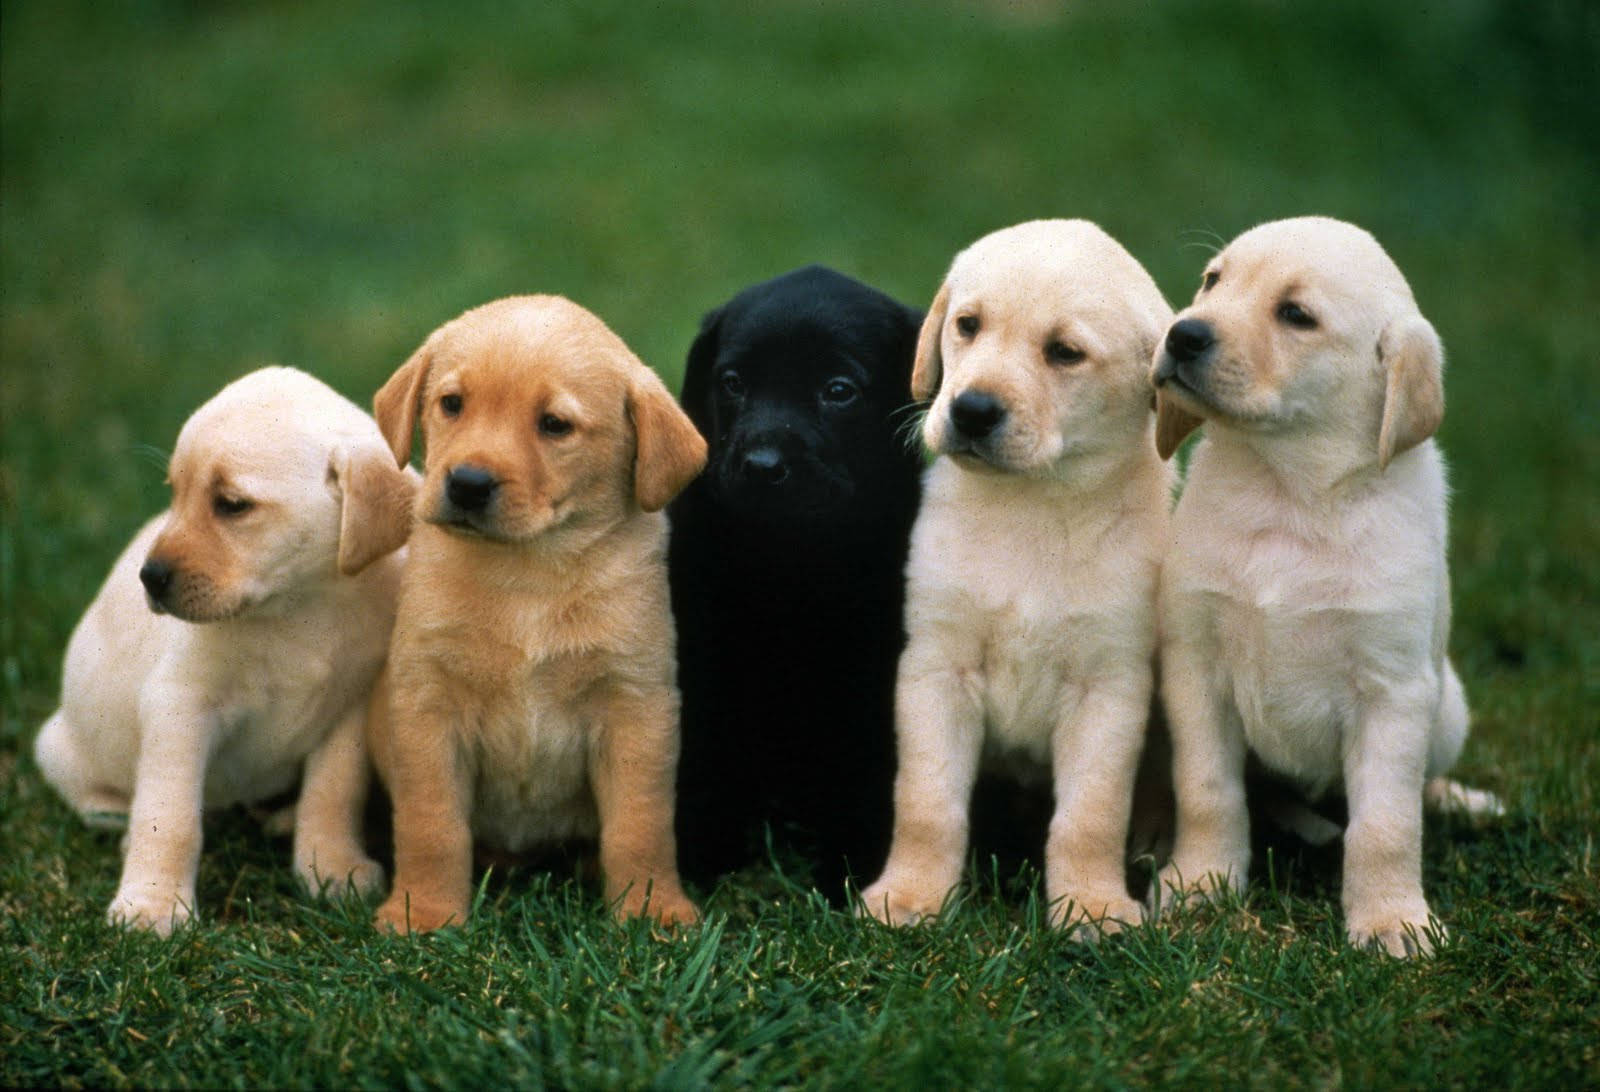
\includegraphics[width=0.35\linewidth]{../5_figuras/fig1}
    \label{fig:a}
    }
    \subfloat [Figura b]{
    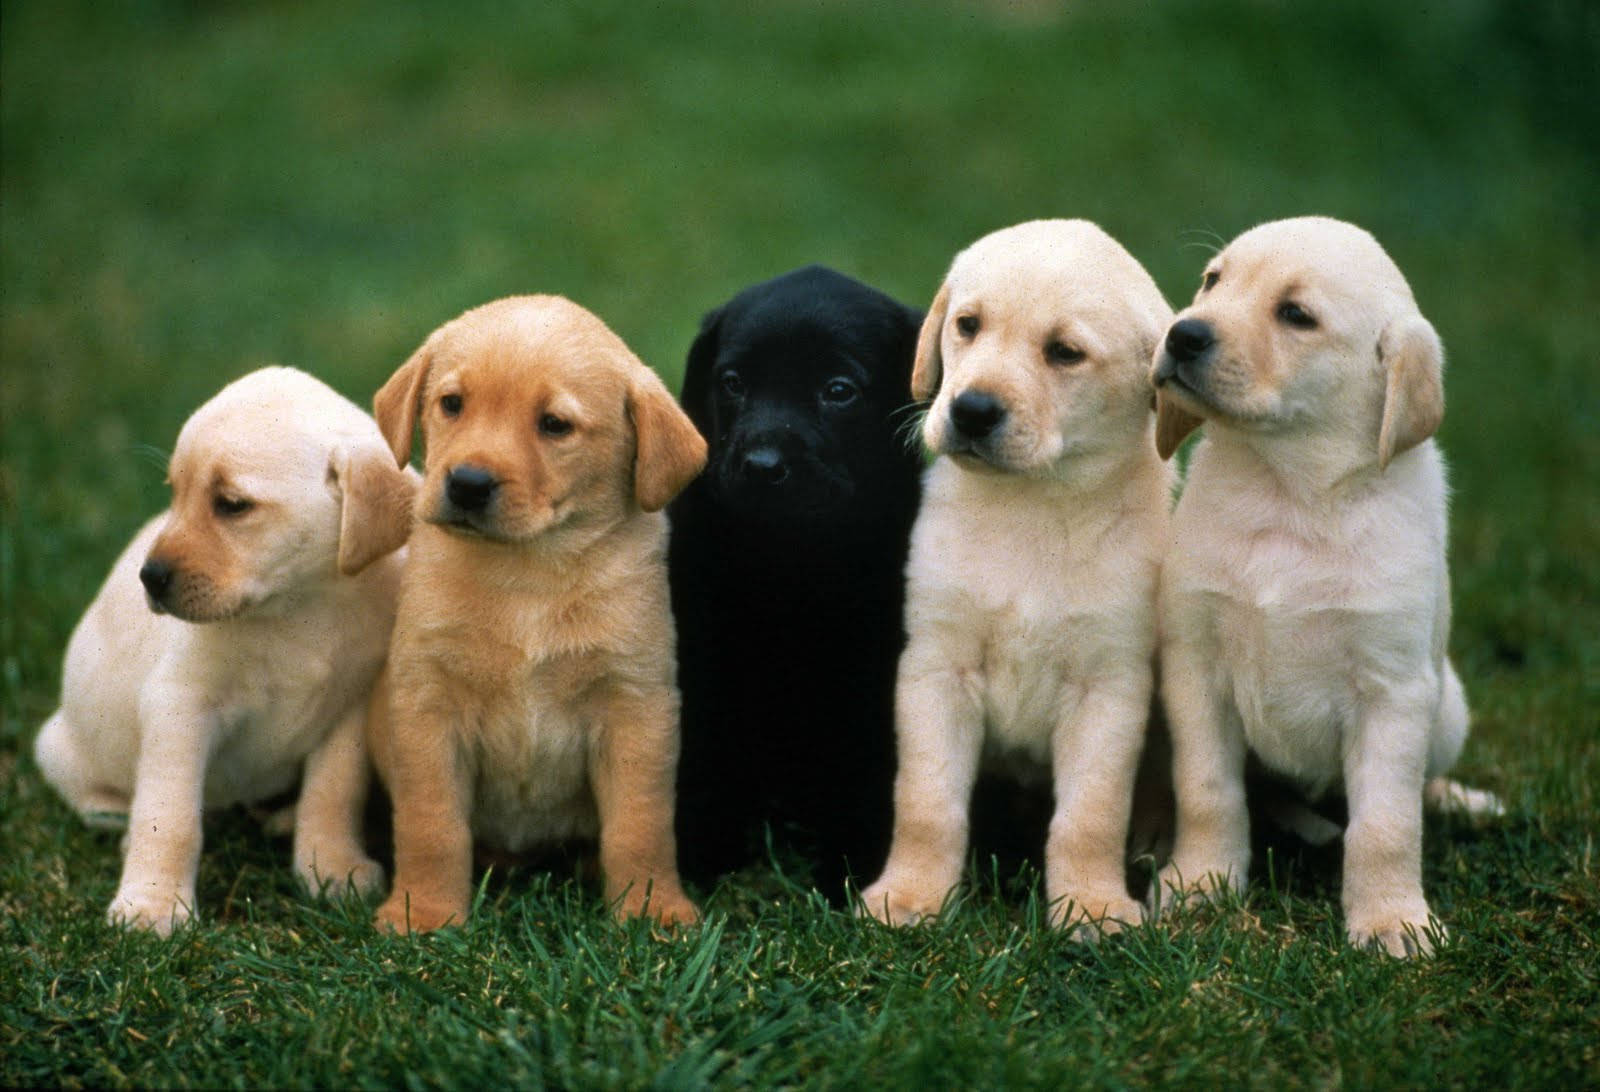
\includegraphics[width=0.35\linewidth]{../5_figuras/fig1}
    \label{fig:b}
    }
    \caption{itulo}
    \end{center}
\end{figure}

\section{Conclus�es do cap�tulo}